\problemname{Gambling Game}
The Ionian Commission on Procuring Cash has come up with a new gambling game to raise funds for the government. The game is played as follows: Each week, the government will televise a set of $m$ balls (numbered $1 \ldots m$) being selected one at a time without replacement. Anyone who wants to play will have to buy a game card. Each card contains $n$ squares (where $n \leq m/2$) and in each square are two numbers between 1 and $m$. No number appears more than once on a card. A sample card is shown in Figure \ref{fig:card}.
\begin{figure}[!h]
\centering
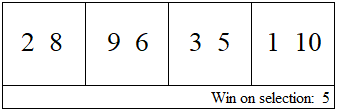
\includegraphics[width=0.5\textwidth]{gamecard}
\caption{Sample game card with $m=10$, $n=4$ and $p=5$.}
\label{fig:card}
\end{figure}

After each ball is selected, players cover any square which contains that number (there will be at most one such square on any card). Each game card also has a number $p$ printed on it, and a contestant wins if he or she covers all $n$ squares after exactly $p$ ball selections (i.e., prior to the $p^{\text{th}}$ selection, they only had $n-1$ squares covered). Before issuing cards to its citizens, the government would like to get an idea of the likelihood of winning for various values of $m, n$ and $p$ so they can set up the payoffs appropriately. They have procured you to write a program to solve this problem.

\section*{Input}
Input consists of a single line containing 3 integers $m, n$ and $p$, as described above, where $2 \leq m \leq 33$, $0 \leq n \leq m/2$ and $0 \leq p \leq m$.

\section*{Output}
Output the probability of winning on the $p^{\text{th}}$ selection as a fraction {\tt x/y} in simplest form. 
